\chapter{Comparison with other known solutions} \label{3}

Two applications that provide similar functionality
and can be compared with this project are Copay \cite{copay} and MyEtherWallet \cite{mew}.
Following sections will provide a brief overview of their features
and how the project tries to improve on them.

\section{Copay}

Copay is a popular application for Bitcoin wallets management.
It's an open source client created by BitPay Inc,
currently featuring hundreds of contributors.
By default, it utilizes Bitcore Wallet Service as its backend
for conntecting to the network, however it can be configured
to integrate with user's custom nodes.

\begin{figure}[ht]
    \centering
    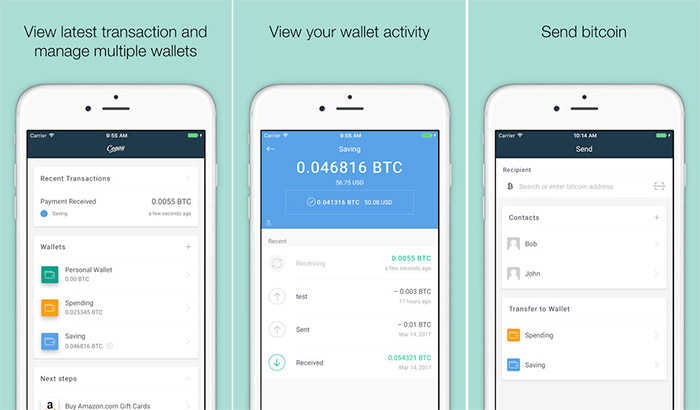
\includegraphics[width=0.7\textwidth]{assets/copay.jpg}
    \caption{Copay interface on a mobile device}
    \label{3:fig:copay}
\end{figure}

\newpage

The application itself is multi-platform, written in JavaScript \cite{javascript}.
On desktop operating systems, it runs on top of Electron \cite{electron}.
It allows for creating wallets, viewing balances and making transfers,
so all the operations considered essential in this thesis are covered.
However the supported currencies currently are Bitcoin and Bitcoin Cash,
which is a fork of Bitcoin -- so in essence just one type of blockchain.
Apparently, the goal here was quality support for few currencies.

The multi-platform nature of the application is quite problematic
on its desktop versions.
The interface is clearly designed mobile-first
and using it with keyboard and mouse is not comfortable.
The screens that the user interacts with display
very limited amounts of information at once,
and accessing some of the less obvious options
often requires traversing several views.
While this kind of design may work well if used on a mobile device,
it does not provide a good user experience for a desktop application.

An interesting fact about Copay is that it has quite recently been
a target of a rather sophisticated attack \cite{copay-attack},
which aimed to steal private keys of users, who possessed more than
100 bitcoins on their wallets.
That incident might have undermined users' trust
in security of the application.

\section{My Ether Wallet}

My Ether Wallet is a wallet management service for Ethereum
and some of the tokens available on its network.
The client is a single page application created in JavaScript
and available under the address \url{https://www.myetherwallet.com}.
The entire project received a design makeover recently,
however its new version does not seem to provide all of the features
available in the previous one yet, so the comparison will be done
in regard to the older version, which is still available at
\url{https://vintage.myetherwallet.com}.

\begin{figure}[ht]
    \centering
    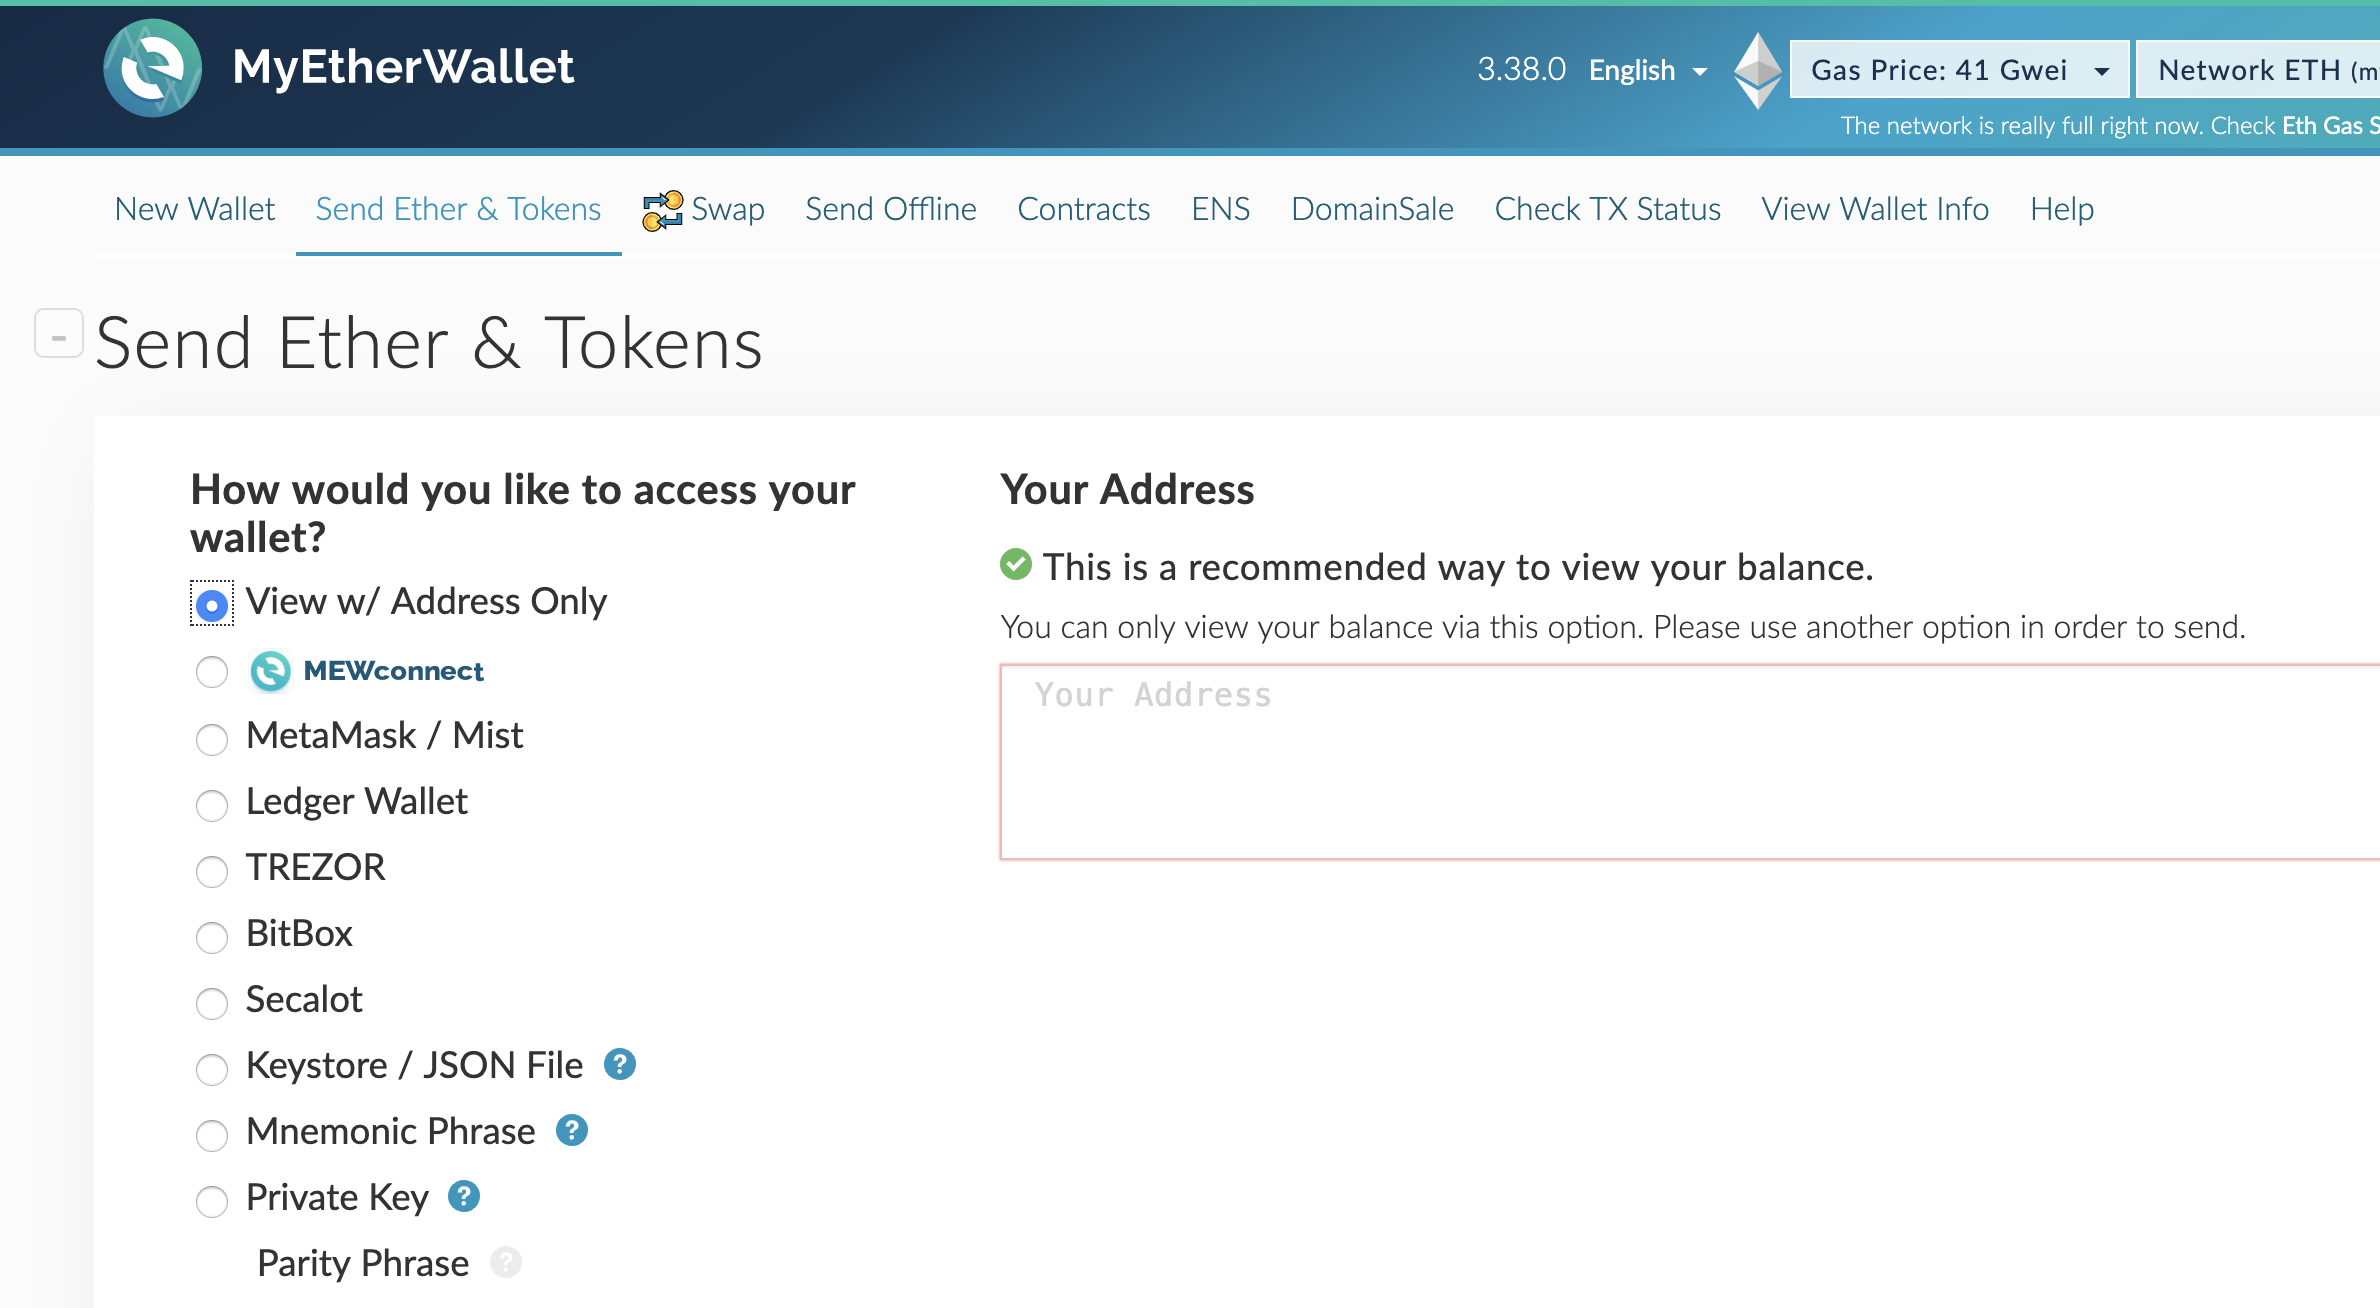
\includegraphics[width=0.7\textwidth]{assets/mew.png}
    \caption{My Ether Wallet website}
    \label{3:fig:mew}
\end{figure}

\newpage

The application is quite feature-rich and allows for connecting
with custom nodes and performing all the necessary operations.
A major advantage is that everything works out of the box
in browser, without the need of installing anything on user's device.

What can be disliked in this application is again the user interface,
although for different reasons than Copay's one.
While this one looks as if it was designed desktop-first, makes good use
of the entire screen and can be comfortably operated with a keyboard and a mouse,
it feels cluttered.
There are too many options displayed on a single screen,
and upon first access an alert with a rather invasive explanation
of how the website works is displayed,
and to make it not appear on user's device
they are forced to read through several screens.

Another major issue with the MyEtherWallet user experience
is that upon refreshing a page, the entire session is lost.
While it might be a good security choice in context of
accessing wallets by their private keys,
it provides a rather poor experience while viewing
wallet by its address.
Not only is the user forced to input it again,
they are also shown the intrusive alert described above
and have to deal with it as well.
